
%(BEGIN_QUESTION)
% Copyright 2010, Tony R. Kuphaldt, released under the Creative Commons Attribution License (v 1.0)
% This means you may do almost anything with this work of mine, so long as you give me proper credit

In this process, two chemical streams are mixed together in a reactor vessel.  The ensuing chemical reaction is endothermic (heat-absorbing) and must be heated by steam to ensure the solution is at the necessary temperature to thoroughly react.  A temperature transmitter (TT) senses the reaction product temperature and sends a 4-20 mA signal to a temperature indicating controller (TIC).  The controller then sends a 4-20 mA control signal to the temperature valve (TV) to throttle steam flow:

$$\includegraphics[width=15.5cm]{i04387x01.eps}$$

First, identify the proper {\it action} of the temperature controller (either direct or reverse) assuming the temperature transmitter is direct-acting, the control valve is fail-open (air-to-close), and the positioner is configured for signal-to-close.

\vskip 10pt

Then explain what would happen if the controller were improperly set for the {\it other} control action.

\vskip 20pt \vbox{\hrule \hbox{\strut \vrule{} {\bf Suggestions for Socratic discussion} \vrule} \hrule}

\begin{itemize}
\item{} What is the opposite of {\it endothermic}, and how might that type of process reactor temperature control be designed differently from this one?
\item{} What would happen to the process temperature if the instrument air supply failed?
\item{} What would happen to the process temperature if the temperature transmitter failed with a low signal?
\item{} What would happen to the process temperature if the positioner's nozzle were to plug?
\item{} How would the controller respond if the steam supply failed?
\item{} How would the controller respond if the condensed water line were to plug?
\end{itemize}

\underbar{file i04387}
%(END_QUESTION)





%(BEGIN_ANSWER)

%(END_ANSWER)





%(BEGIN_NOTES)

The controller should be configured for {\it direct} action.  If it were mis-configured for reverse action, the process temperature would either become far too cold or far too hot, depending on where the temperature was in relation to setpoint at the time of the controller mis-configuration.

\vfil \eject

\noindent
{\bf Prep Quiz:}

Determine the proper controller actions required in this process, assuming direct-acting transmitters and signal-to-open control valves:

$$\includegraphics[width=15.5cm]{i04387x02.eps}$$

Temperature controller = {\it direct} or {\it reverse}?

\vskip 10pt

Pressure controller = {\it direct} or {\it reverse}?

\vfil \eject

\noindent
{\bf Prep Quiz:}

Determine the proper controller actions required in this process, assuming direct-acting transmitters and signal-to-close control valves:

$$\includegraphics[width=15.5cm]{i04387x02.eps}$$

Temperature controller = {\it direct} or {\it reverse}?

\vskip 10pt

Pressure controller = {\it direct} or {\it reverse}?


%INDEX% Basics, control loop troubleshooting: determining effect of specified fault(s)
%INDEX% Process: steam-heated reactor vessel (generic)

%(END_NOTES)


